% !TEX encoding = UTF-8 Unicode
\documentclass{beamer}
% \usetheme{Luebeck}
\usetheme{Frankfurt}
\usecolortheme{default}
\setbeamercolor{bibliography entry author}{fg=black}
\beamertemplatenavigationsymbolsempty

\usepackage[english,serbian]{babel}
\usepackage[utf8]{inputenc}
\usepackage{color}
\usepackage{url}
\usepackage{graphicx}
\usepackage{amsmath}
\usepackage{amsfonts}
\graphicspath{ {images/} }

\DeclareMathOperator*{\argmax}{argmax}

\title{Automatsko prepoznavanje govora}
\subtitle{Seminarski rad u okviru kursa\\Metodologija stručnog i naučnog rada}
\author[Vladimir Vuksanović, Aleksa Kojadinović, Lazar Čeliković]{
  \texorpdfstring{Vladimir Vuksanović, vladevuksan99@gmail.com\\Aleksa Kojadinović, kojadinovic.aleksa98@gmail.com\\Lazar Čeliković, celikoviclazar@hotmail.com}
  {Vladimir Vuksanović, Aleksa Kojadinović, Lazar Čeliković}
}
\institute{Matematički fakultet}
\date{\today}

\begin{document}

\frame{\titlepage}

\begin{frame}{Sadržaj}
  \tableofcontents[hideallsubsections]
\end{frame}

\section{Uvod}
\begin{frame}
  \frametitle{Uvod}

  \begin{itemize}
    \item \textbf{Automatsko prepoznavanje govora} (eng.~{\em Automatic Speech Recognition, ASR}) je proces pretvaranja zvučnog signala govora u odgovarajući niz reči pomoću računara
    \item Neke od najznačajnijih primena su:
    \begin{itemize}
      \item pametni lični asistenti (Google Assistant, Apple Siri, \dots)
      \item transkripcija i pretraživanje audio sadržaja
      \item automatsko titlovanje snimaka
      \item pristupačnost (eng.~{\em accessibilty})
    \end{itemize} 
  \end{itemize}
\end{frame}

\section{Izazovi}
\begin{frame}
  \frametitle{Izazovi}

  \begin{enumerate}
    \item Mala količina podataka za trening
    \item Stil govora
    \begin{itemize}
      \item Izolovane reči
      \item Povezane reči
      \item Neprekidan govor
      \item Spontani govor
    \end{itemize}
    \item Karakteristike govornika (pol, starost, brzina govora...)
    \item Okruženje govornika (pozadinska buka, oprema za snimanje)
    \item Veličina rečnika
  \end{enumerate}
\end{frame}

\section{Statistički model}

\subsection{Statistički model}
\begin{frame}
  \frametitle{Statistički model}

  \begin{itemize}
    \item Koriste statističke metode za određivanje najverovatnije transkripcije
    \item Ako je $X$ ulazni zvuk, traži se najverovatniji niz reči $\hat{W} \approx \argmax_{W,S} P(X|S) P(S|W) P(W)$
  \end{itemize}

  \begin{figure}
    \begin{center}
    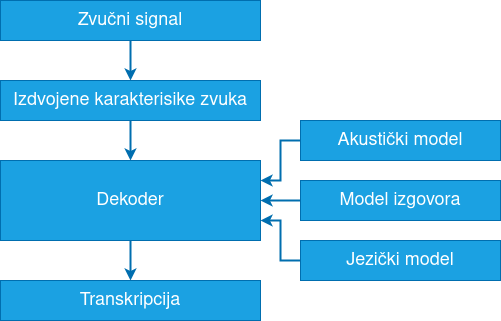
\includegraphics[scale=0.39]{statistical_model.png}
    \end{center}
    \caption{Struktura statističkog modela}
  \end{figure}
\end{frame}

\subsection{Akustički model i model izgovora}
\begin{frame}
  \frametitle{Akustički model i model izgovora}

  \begin{itemize}
    \item Akustički model 
    \begin{itemize}
      \item Predviđa verovatnoće koliko ulazni zvuk odgovara nizu fonema
      \item Foneme su najmanje jezičke jedinice na osnovu kojih mogu da se razlikuju značenja većih jedinica
      \item Implementiran skrivenim Markovljevim modelom
    \end{itemize}
    \item Model izgovora
    \begin{itemize}
      \item Mapira reči u njihov način izgovora (fonetski zapis)
      \item Definisan od strane eksperta za jezik
      \item Određuje način povezivanja modela fonema u model reči
    \end{itemize}
  \end{itemize}

  \begin{figure}
    \begin{center}
    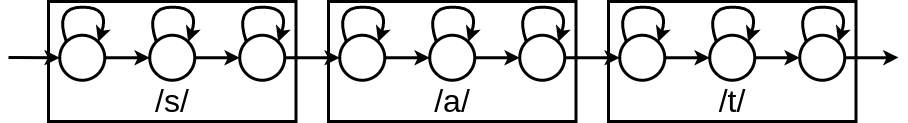
\includegraphics[scale=0.3]{word_hmm.png}
    \end{center}
    \caption{Primer skrivenog Markovljenog modela za reč ``sat''}
  \end{figure}
\end{frame}

\subsection{Jezički model}
\begin{frame}
  \frametitle{Jezički model}

  \begin{itemize}
    \item Određuje verovatnoću predviđanja rečenice na osnovu:
    \begin{itemize}
      \item relativne učestalosti reči
      \item redosleda reči
      \item sintaksne ispravnosti
      \item semantičke ispravnosti
    \end{itemize}
    \item Implementiran pomoću n-grama
    \item Dužina n-grama je obično 3 i smanjuje se dok se ne pronađe prvo pojavljivanje u trening skupu
  \end{itemize}
\end{frame}

\section{End-to-end model}
\subsection{End-to-end model}
\begin{frame}
  \frametitle{End-to-end model}
  \begin{itemize}
    \item Zasnovan na dubokim neuronskim mrežama 
    \item Ima prostiju strukturu od statističkog modela
    \item On se bavi direktnim prevođenjem ulaznog signala u niz grafema, karatera ili reči
    \item Treniranje postaje lakše zbog jednostavnije strukture
    \item Sa druge strane potrebna je veća količina podataka nego ako se koristi statistički model
    \item U odnosu na način rešavanja, razlikujemo \textbf{CTC model} \cite{graves2006ctc} i \textbf{model zasnovan na pažnji} \cite{chorowski2015attentionbased}
  \end{itemize} 
\end{frame}

\subsection{CTC (Connectionist Temporal Classification)}
\begin{frame}
  \frametitle{CTC (Connectionist Temporal Classification)}
  \begin{itemize}
    \item Cilj je napraviti preslikavanje $h$ koje slika proizvoljan zvučni signal u niz labela:
      \begin{equation*}
      h: (\mathbb{R}^m)^* \rightarrow L^* 
      \end{equation*}
    \item Ako $O$ označava test skup, tada se funkcija greške definiše na sledeći način:
      \begin{equation*}
      LER(h, O) = \frac{1}{|O|}\sum_{(\textbf{x}, \textbf{z}) \in O}\frac{ED(h(\textbf{x}), \textbf{z})}{|\textbf{z}|}
      \end{equation*}
    \item Implementiran kao rekurentna neuronska mreža koja za svaki od $T$ trenutaka ima $m$ ulaza, a izlaz je softmax sloj dimenzije $|L'|$, gde je $L'$ azbuka proširena blanko karakterom
  \end{itemize}  
\end{frame}

\subsection{Modeli zasnovani na pažnji}
\begin{frame}
  \frametitle{Modeli zasnovani na pažnji}
  \begin{itemize}
      \item Za razliku od CTC modela, ovi modeli se oslanjaju na \textbf{mehanizam pažnje} (eng.~{\em attention mechanism}) i odbacuju pretpostavku o nezavisnosti zvučnih segmenata
      \item Glavne komponente ovog modela su:
        \begin{itemize} 
          \item \textbf{Slušalac} -- rekurentna neuronska mreža piramidalne strukture čiji zadatak je da napravi reprezentaciju zvuka višeg nivoa
          \item \textbf{Speler} -- rekurentna neuronska mreža koja proizvodi konačan niz karaktera
        \end{itemize}
      \item Koristeći koncepte stanja i konteksta, verovatnoća odabira narednog karaktera zavisi od svih prethodnih karaktera
  \end{itemize}
\end{frame}

\section{Metrike za evaluaciju}
\begin{frame}
  \frametitle{Word Error Rate (WER)}

  \begin{equation*}
    WER = \frac{I + D + S}{N}
  \end{equation*}
  gde je:
  \begin{itemize}
    \item $I$ broj umetnutih reči
    \item $D$ broj obrisanih reči
    \item $S$ broj zamenjenih reči
    \item $N$ ukupan broj reči u referenci
  \end{itemize}
\end{frame}

\section{Literatura}
\begin{frame}{Literatura}
    \bibliography{presentation} 
    \bibliographystyle{ieeetr}
\end{frame}

\end{document}